\documentclass[tikz,border=10pt]{standalone}
\usepackage{enumitem} % For compact itemize lists
\usetikzlibrary{arrows.meta, positioning, shadows}

\definecolor{uzkblau}    {RGB} {0,81,118}

\begin{document}

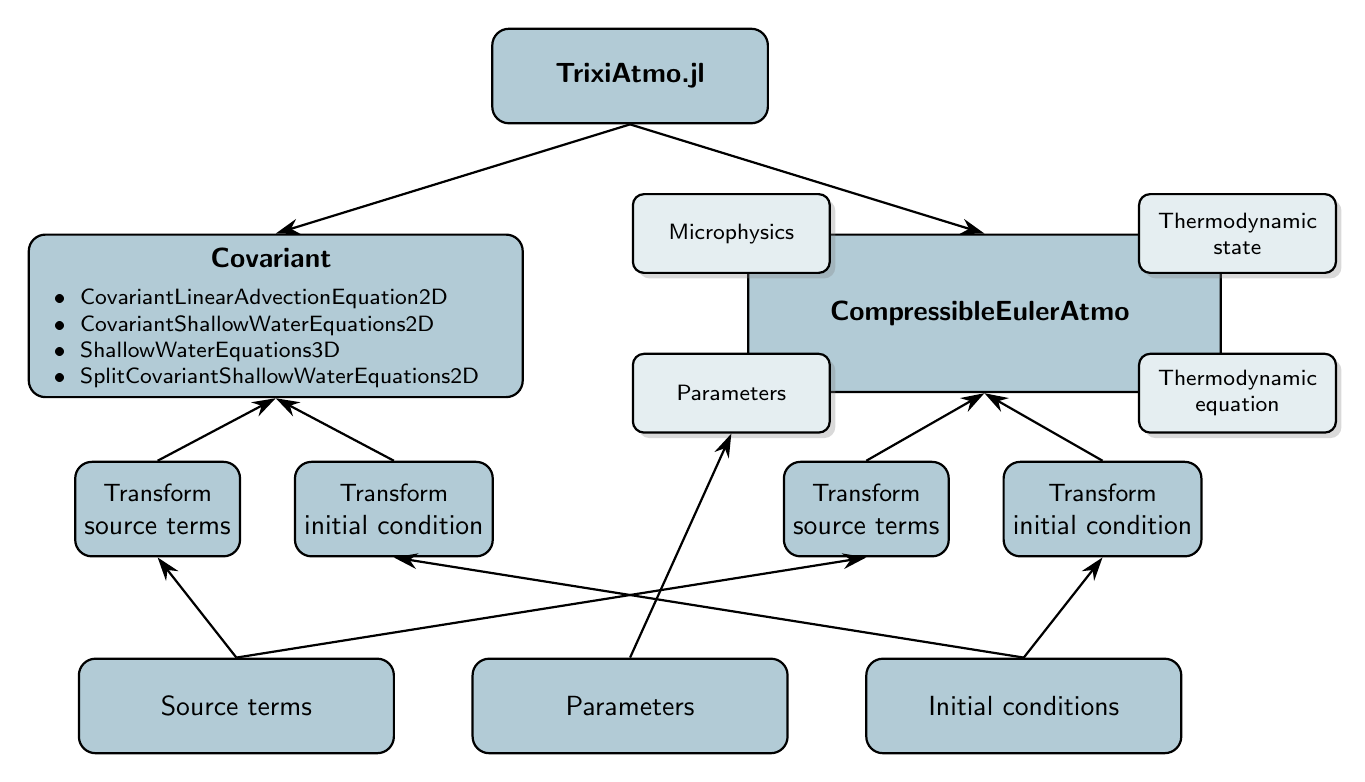
\begin{tikzpicture}[
    % Define the style for the tiles
    tile/.style={
        rectangle,
        rounded corners=6pt,
        draw=black,
        thick,
        fill=uzkblau!30,
        align=center,
        minimum height=1.2cm,
        font=\sffamily
    },
    % Define the style for the arrows
    arrow/.style={
        ->,
        thick,
        >={Stealth[length=3mm, width=2mm]}
    }
]

    % ---------------------------------------------------
    % 1. MAIN CENTER NODE
    % ---------------------------------------------------
    \node[tile, minimum width=3.5cm] (trixi) at (0, 0) {\textbf{TrixiAtmo.jl}};

    % ---------------------------------------------------
    % 2. SOUTH-WEST NODE (Cartesian + 4 Overlapping Tiles)
    % ---------------------------------------------------
    % Main Cartesian Node (now with a shadow)
    \node[
        tile,
        anchor = north,
        align = center,
        minimum height=2cm,
        minimum width=6cm,
    ] (cartesian) at (4.5, -2.0) {
        \textbf{CompressibleEulerAtmo}
    };

    % 4 Overlapping Tiles
    % We use a scope to define a localized style for these smaller tiles
    \begin{scope}[
        subtile/.style={
            rectangle,
            rounded corners=4pt,
            draw=black,
            thick,
            fill=uzkblau!10, % White fill so it contrasts against the blue main tile
            align=center,
            font=\sffamily\footnotesize,
            minimum width=2.5cm,
            minimum height=1.0cm,
            drop shadow={opacity=0.3, shadow xshift=2pt, shadow yshift=-2pt}
        }
    ]
        % Placed on the 4 corners.
        % You can adjust the xshift and yshift to control exactly how much they overlap!
        \node[subtile] at ([xshift=-0.2cm, yshift=0.0cm]cartesian.north west) {Microphysics};
        \node[subtile] at ([xshift=0.2cm, yshift=0.0cm]cartesian.north east)  {Thermodynamic\\state};
        \node[subtile] (cartesian_par) at ([xshift=-0.2cm, yshift=0.0cm]cartesian.south west){Parameters};
        \node[subtile] at ([xshift=0.2cm, yshift=0.0cm]cartesian.south east) {Thermodynamic\\equation};
    \end{scope}


    % Covariant Node (South-East)
    \node[tile,anchor=north] (covariant) at (-4.5, -2.0) {
        \begin{tabular}{c}
            \textbf{Covariant} \\[1ex]
            \begin{minipage}{5.5cm}
               \footnotesize
               \begin{itemize}[leftmargin=*, nosep]
                    \item CovariantLinearAdvectionEquation2D
                    \item CovariantShallowWaterEquations2D
                    \item ShallowWaterEquations3D
                    \item SplitCovariantShallowWaterEquations2D
                \end{itemize}
            \end{minipage}
        \end{tabular}
    };

    \node[tile] (covariant_trafo_ic) at (-3.0, -5.5) {\small Transform\\initial condition};
    \node[tile] (covariant_trafo_st) at (-6.0, -5.5) {\small Transform\\source terms};

    \node[tile] (cartesian_trafo_ic) at (6.0, -5.5) {\small Transform\\initial condition};
    \node[tile] (cartesian_trafo_st) at (3.0, -5.5) {\small Transform\\source terms};

    % ---------------------------------------------------
    % BOTTOM
    % ---------------------------------------------------
    \node[tile, minimum width=4cm] (ic) at (5, -8) {Initial conditions};
    \node[tile, minimum width=4cm] (st) at (-5, -8) {Source terms};
    \node[tile, minimum width=4cm] (par) at (0, -8) {Parameters};

    % ---------------------------------------------------
    % 5. ARROWS
    % ---------------------------------------------------
    % Arrows leaving TrixiAtmo.jl (South-East and South-West)
    \draw[arrow] (trixi.south) -- (cartesian.north);
    \draw[arrow] (trixi.south) -- (covariant.north);

    % Arrows from left tiles pointing towards the middle
    \draw[arrow] (covariant_trafo_ic.north) -- (covariant.south);
    \draw[arrow] (covariant_trafo_st.north) -- (covariant.south);

    % Arrows from right tiles pointing towards the middle
    \draw[arrow] (cartesian_trafo_ic.north) -- (cartesian.south);
    \draw[arrow] (cartesian_trafo_st.north) -- (cartesian.south);

    % Arrows from bottom tiles
    \draw[arrow] (ic.north) -- (covariant_trafo_ic.south);
    \draw[arrow] (ic.north) -- (cartesian_trafo_ic.south);
    \draw[arrow] (st.north) -- (covariant_trafo_st.south);
    \draw[arrow] (st.north) -- (cartesian_trafo_st.south);
    \draw[arrow] (par.north) -- (cartesian_par.south);

\end{tikzpicture}

\end{document}
